\chapter{تحلیل، طراحی و پیاده‌سازی سیستم}
در این فصل به توضیحات مربوط به تحلیل، طراحی و پیاده‌سازی سیستم پرداخته می‌شود. ابتدا متدولوژی مورد استفاده در این سیستم توضیح داده شده و سپس نیازمندی‌های سیستم بررسی می‌شوند. در ادامه با معماری این سیستم و بخش‌های مختلف آن آشنا شده و چگونگی پیاده‌سازی هر یک از بخش‌های سیستم جداگانه توضیح داده می‌شود.

\section{الگوی سیستم}
یک متدولوژی مجموعه‌ای از روش‌ها، توصیه‌ها و قالب‌ها است که به همراه راهبرد مشخص و طی مراحل مختلف، در توسعه‌ی سیستم به‌کار گرفته می‌شود. براساس رویکرد‌های مختلف متدولوژی‌های مختلفی وجود دارد. به‌عنوان مثال در رویکرد توسعه چابک\footnote{\lr{Agile}}، متدولوژی‌های اسکرام\footnote{\lr{Scrum}} و کانبان\footnote{\lr{Kanban}} وجود دارند. یا در رویکرد شیءگرا\footnote{\lr{Object Oriented}} متدولوژی \lr{RUP}\footnote{\lr{Rational Unified Process}} تعریف شده است. انتخاب متدولوژی وابسته به عوامل بسیاری چون نیازمندی‌های نرم‌افزار، تعداد اعضاء تیم، زمان‌بندی پروژه و ... می‌باشد. 
از آنجا که نیازمندی‌های سیستم به طور دقیق در ابتدا مشخص نبوده‌اند از الگوی چابک\footnote{\lr{Agile}} استفاده شده است. این الگو در واقع همان الگوی آبشاری\footnote{\lr{Waterfall Model}} است که در چندین تناوب تکرار می‌شود و ‌مراحل پیاده‌سازی و آزمایش همزمان با مراحل تحلیل و طراحی سیستم مورد نظر انجام می‌گیرد. در این الگو هر آنچه تولید می‌شود بلافاصله مورد آزمایش قرار می‌گیرد و سپس با تحلیل دوباره‌ی نیازمندی‌ها مراحل تکرار می‌شوند \cite{pressman2019software}. در الگوی چابک استفاده شده در این پروژه، مراحل زیر به ترتیب و به صورت تکرارشونده انجام شده‌اند:
\begin{enumerate}
	\item تحلیل نیازمندی‌ها
	\item برنامه‌ریزی
	\item طراحی سیستم
	\item پیاده‌سازی
	\item آزمایش‌
\end{enumerate}

در ادامه توضیحات مربوط به تحلیل، طراحی و پیاده‌سازی نرم‌افزار آورده شده‌ است. توضیحات مربوط به آزمایش و اعتبارسنجی قسمت‌های مختلف سیستم در فصل‌های مربوط به خودشان توضیح داده خواهد شد.

\section{تحلیل نیازمندی‌های سیستم}

این سیستم دو دسته استفاده کننده دارد.
دسته‌ی اول کاربر عادی سیستم است که نیازمندی‌های آن به شرح زیر است:

\begin{itemize}
	\item ورود سوال: کاربر عادی باید بتواند یک جمله را به عنوان پرسش مورد نظرش در سیستم ثبت کند تا سیستم آنرا بررسی کند.
	\item دریافت پاسخ: کاربر عادی باید بتواند پاسخ‌هایی که سیستم بدست آورده را مشاهده نماید.
	\item دریافت پاسخ‌های غیرمنتخب: این کاربر باید بتواند پاسخ‌های غیرمنتخب تشخیص داده شده توسط سیستم را مشاهده کند. این نیازمندی زیرمجموعه‌ی نیازمندی دریافت پاسخ می‌باشد. 
\end{itemize}
دسته‌ی دوم کاربر تحلیل‌گر است. تحلیل‌گر تمامی نیازمندی‌های ذکر شده برای کاربر عادی را شامل شده و نیازمندی‌های زیر را نیز دارد:

\begin{itemize}
	\item احراز هویت: تحلیل‌گر باید بتواند خود را به سیستم بشناساند و تحت عنوان تحلیل‌گربه سیستم ورود یا خروج کند. 
	\item دریافت اطلاعات میانی: تحلیل‌گر می‌تواند اطلاعات میانی سیستم که شامل کوئری‌های ارسال شده توسط سیستم است را مشاهده نماید.
\end{itemize}
نیازمندی‌های کاربردی سیستم توسط نمودار \lr{Use case} نمایش داده می‌شود. در شکل \ref{fig:use_case} این نمودار را مشاهده می‌کنید. همانطور که گفته شد این سیستم دارای دو نقش کاربر عادی و تحلیل‌گر می‌باشد.

\begin{figure}[t!]
	\centering
	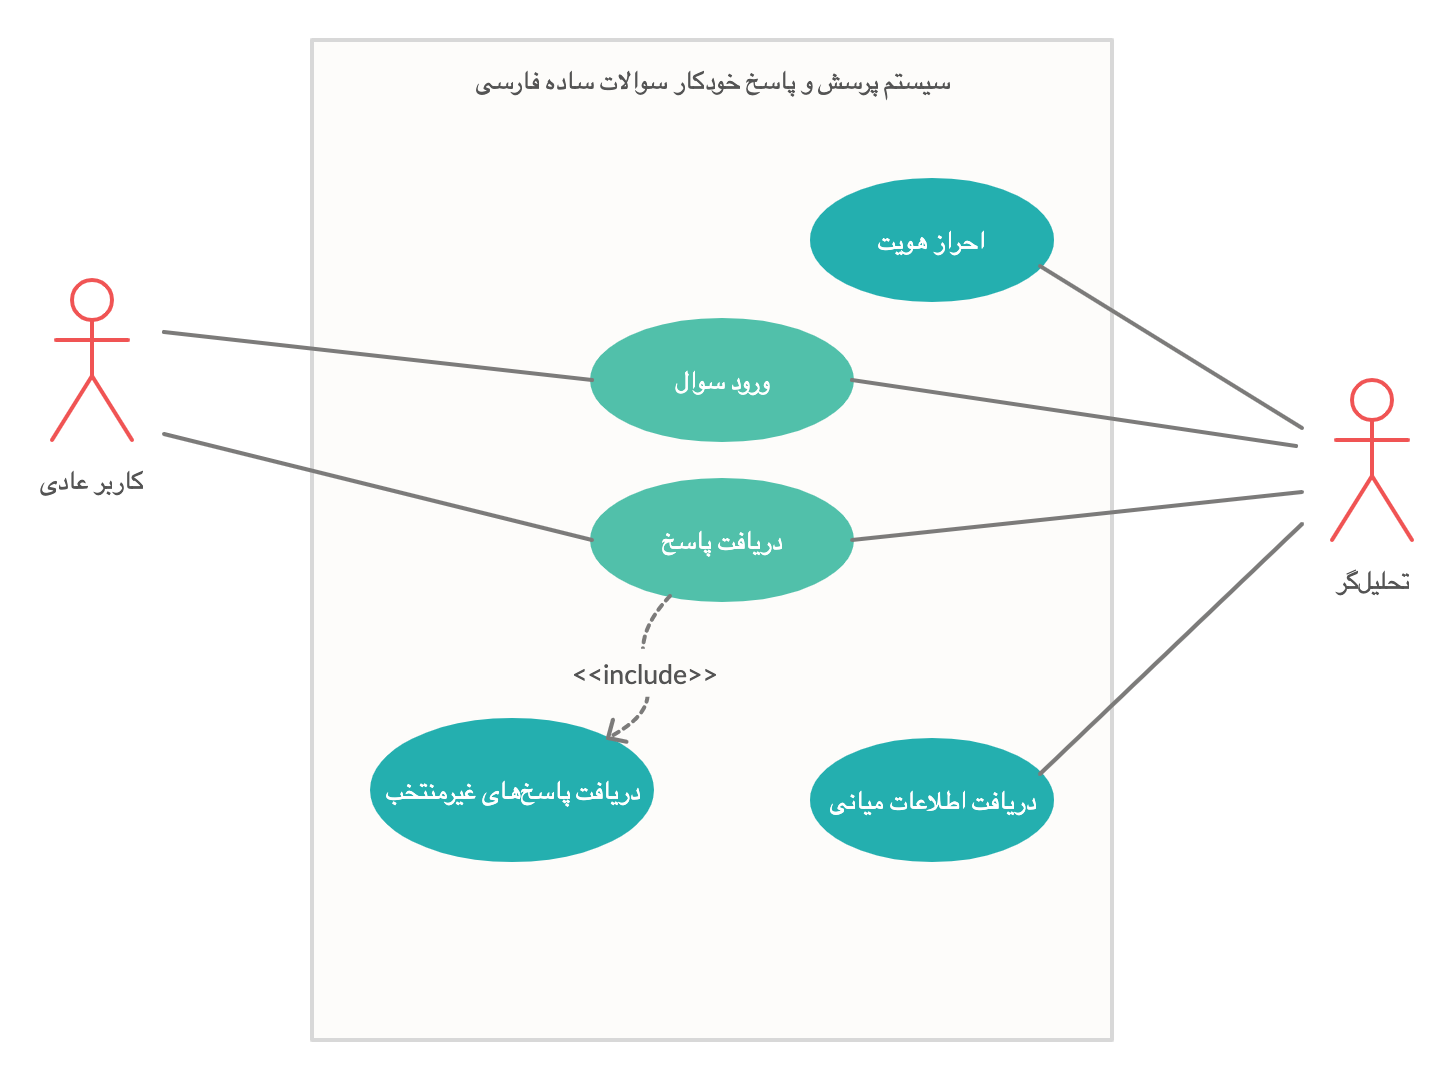
\includegraphics[width=15cm]{figures/se-diagrams/use-case.png}
	\caption[نمودار \lr{Use case}]{نمودار \lr{Use case}}
	\label{fig:use_case}
\end{figure}

\section{طراحی سیستم}
در شکل \ref{fig:architecture}  معماری این سیستم را مشاهده می‌کنید که از الگوی سرویس‌دهنده-سرویس‌گیرنده برای طراحی آن استفاده شده است.
این سیستم بوسیله‌ی یک رابط کاربری تحت وب برای کاربر ارائه می‌شود. بنابراین بخش‌های اصلی سیستم شامل بخش سرویس‌دهنده و سرویس‌گیرنده می‌باشد.
بخش سرویس‌دهنده دارای سه بخش اصلی هسته سیستم، سرویس وب و اتصال به پایگاه دانش می‌باشد. هسته سیستم بخش اصلی سیستم است و شامل مدل‌های یادگیری ماشین برای تشخیص رابطه و موجودیت‌های داخل سوال بوده و وظیفه‌ی تولید کوئری مرتبط را نیز دارد. بخش اتصال به پایگاه داده وظیفه‌ی ارسال کوئری و گرفتن پاسخ از گراف دانش را انجام می‌دهد. 
کاربر بوسیله‌ی رابط کاربری تحت وب با سرویس‌گیرنده و سرویس‌گیرنده بوسیله‌ی سرویس وب با سرویس‌دهنده در ارتباط است.

\begin{figure}[t!]
	\centering
	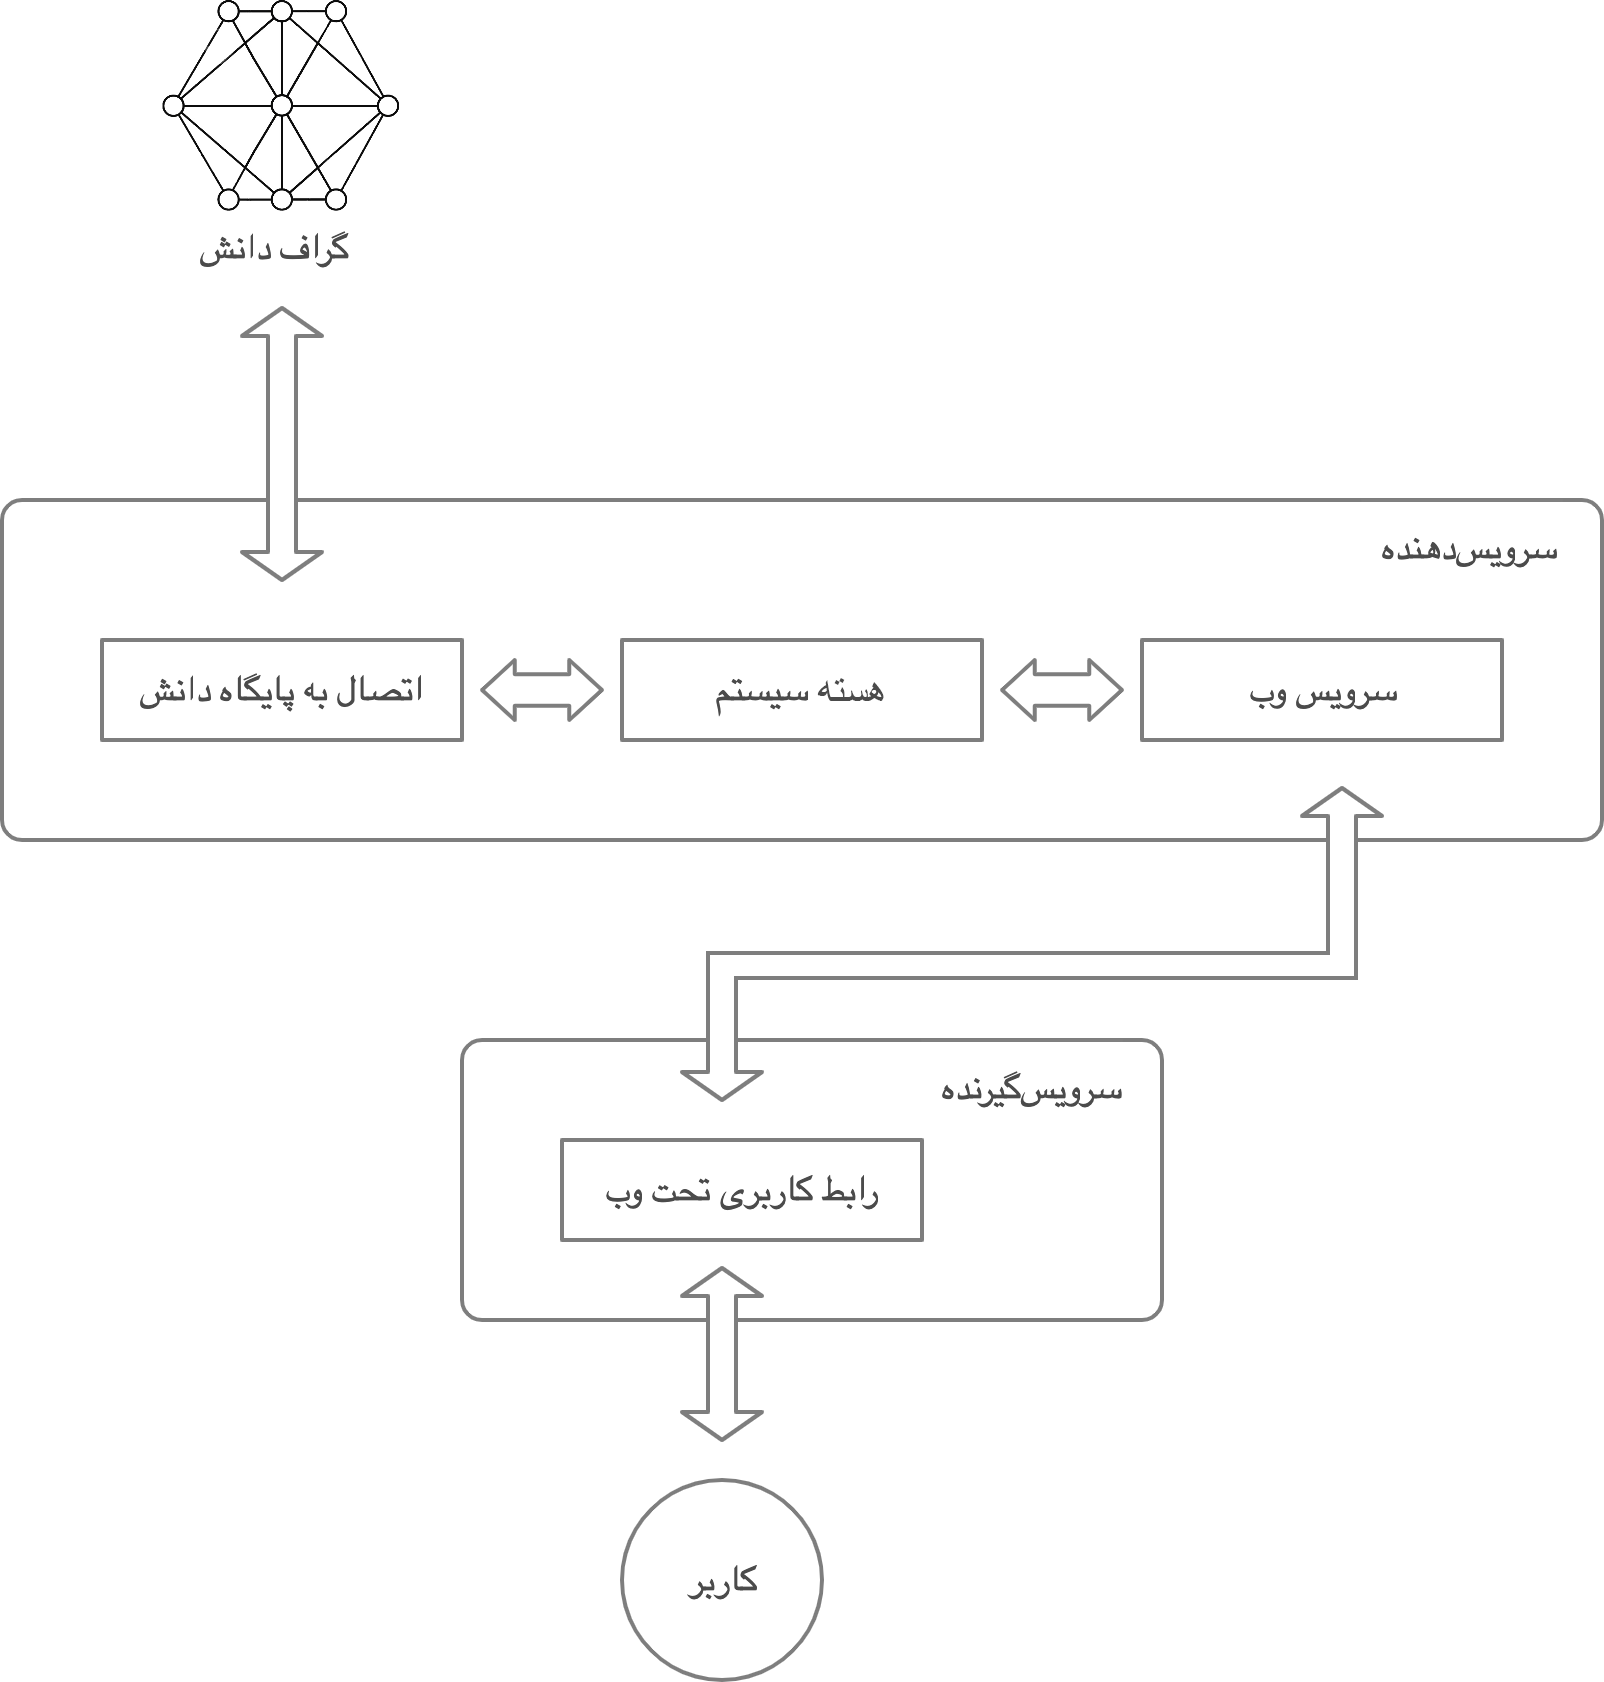
\includegraphics[width=12cm]{figures/se-diagrams/architecture.png}
	\caption[معماری سیستم]{معماری سیستم}
	\label{fig:architecture}
\end{figure}


\section{پیاده‌سازی سیستم}

بخش عمده‌ی این سیستم بوسیله‌ی زبان پایتون\footnote{\lr{Python}} نسخه‌ی ۳.۶.۷ پیاده‌سازی شده است. در این بخش هر کدام از قسمت‌های سیستم که در بخش طراحی ذکر شده‌اند توضیح داده خواهند شد.

\subsection{هسته سیستم}
هسته سیستم بخش اصلی این سیستم است که وظیفه‌ی آن پاسخ‌دهی به سه زیرمسئله‌ی اصلی سیستم شامل تشخیص رابطه، تشخیص موجودیت و تولید کوئری می‌باشد. این بخش همان سیستم پیشنهادی توضیح داده شده در فصل پیشین است.
فایل اصلی این قسمت \lr{answer\_generator.py} است که وظیفه‌ی آن آماده‌سازی روند پاسخ‌دهنده‌ی سوالات کاربران می‌باشد. در این فایل روندهای مورد نیاز برای سه زیرمسئله‌ی بیان شده فراخوانی شده و استفاده می‌شوند.
\subsection{اتصال به پایگاه دانش}
در فصل قبل چگونگی تولید کوئری مورد نیاز برای ارسال به پایگاه دانش فارس‌بیس شرح داده شد. بخش اتصال به پایگاه دانش وظیفه دارد که کوئری‌های تولید شده توسط سیستم را به پایگاه دانش ارسال کرده و پاسخ مرتبط را از پایگاه دریافت نموده و به سیستم بازگرداند. پایگاه دانش فارس‌بیس چنین درخواست‌هایی را از طریق آدرس \lr{http://farsbase.net:8890/sparql} پاسخ می‌دهد. این درخواست‌ها با استفاده از متد \lr{Post} در پروتکل \lr{HTTP} ارسال می‌شوند. پاسخ دریافتی از پایگاه دانش که به صورت \lr{XML} است می‌تواند در برگیرنده‌ی چندین موجودیت به عنوان پاسخ باشد. این موجودیت‌ها می‌توانند دارای گره در پایگاه دانش باشند که در این صورت آدرس آنها در پایگاه بازگردانده می‌شود.
روندهای مربوط به این قسمت در فایل \lr{graph\_extractor.py} پیاده‌سازی شده‌اند.
\subsection{سرویس و رابط کاربری تحت وب}
تمامی فایل‌های مربوط به این دو بخش از سیستم در پکیج \lr{web\_interface} قرار دارند.
\subsubsection{سرویس}
برای اتصال هسته سیستم به رابط کاربری وب از کتابخانه‌ی \lr{Flask} در پایتون استفاده شده است. بوسیله‌ی این کتابخانه رابطهای برنامه‌نویسی کاربردی مورد نیاز فراهم شده و بوسیله‌ی آنها روندهای متناسب در هسته سیستم فراخوانی می‌شوند.\\
دو مسیر\footnote{\lr{Route}} در این سرویس ارائه می‌شود. مسیر اول به آدرس \lr{"/"} صفحه‌ی اصلی رابط کاربری را برای کاربر نمایش می‌دهد که کاربر می‌تواند در این صفحه پرسش مورد نظر خود را وارد کرده و پاسخ را مشاهده کند. مسیر دوم به آدرس \lr{"/answer"} می‌تواند بوسیله‌ی متد\footnote{\lr{Method}} \lr{Post} در پروتکل \lr{HTTP} فراخوانی شود. این مسیر پرسش وارد شده توسط کاربر را همراه با پارامترهای دیگر دریافت کرده و با فراخوانی روند مورد نیاز در هسته سیستم پاسخ را در فرمت \lr{JSON} برمی‌گرداند.\\
این سرویس در فایل \lr{interface.py} پیاده‌سازی شده است.
\subsubsection{رابط کاربری}
در رابط کاربری کاربران می‌توانند پرسش خود را وارد کنند و رابطه و موجودیت تشخیص داده شده برای آن و پاسخ خود را دریافت نمایند. رابط کاربری تحت وب با فراخوانی رابطهای برنامه‌نویسی کاربردی پیاده‌سازی شده در سرویس وب با سرویس‌دهنده ارتباط برقرار می‌کند. برای کاربران این گزینه وجود دارد که اگر بخواهند سیستم روابط غیر منتخب را نیز برایشان بررسی کند که در این صورت احتمال درستی هر کدام از روابط تشخیص‌ داده شده نیز نمایش داده می‌شود. کاربر تحلیل‌گر می‌تواند اطلاعات میانی سیستم که شامل کوئری ارسالی می‌شود را نیز مشاهده کند. تصاویری از رابط کاربری را همراه با پرسش‌ها و حالات مختلف مشاهده می‌کنید.
\vfill
\begin{figure}[h]
	\centering
	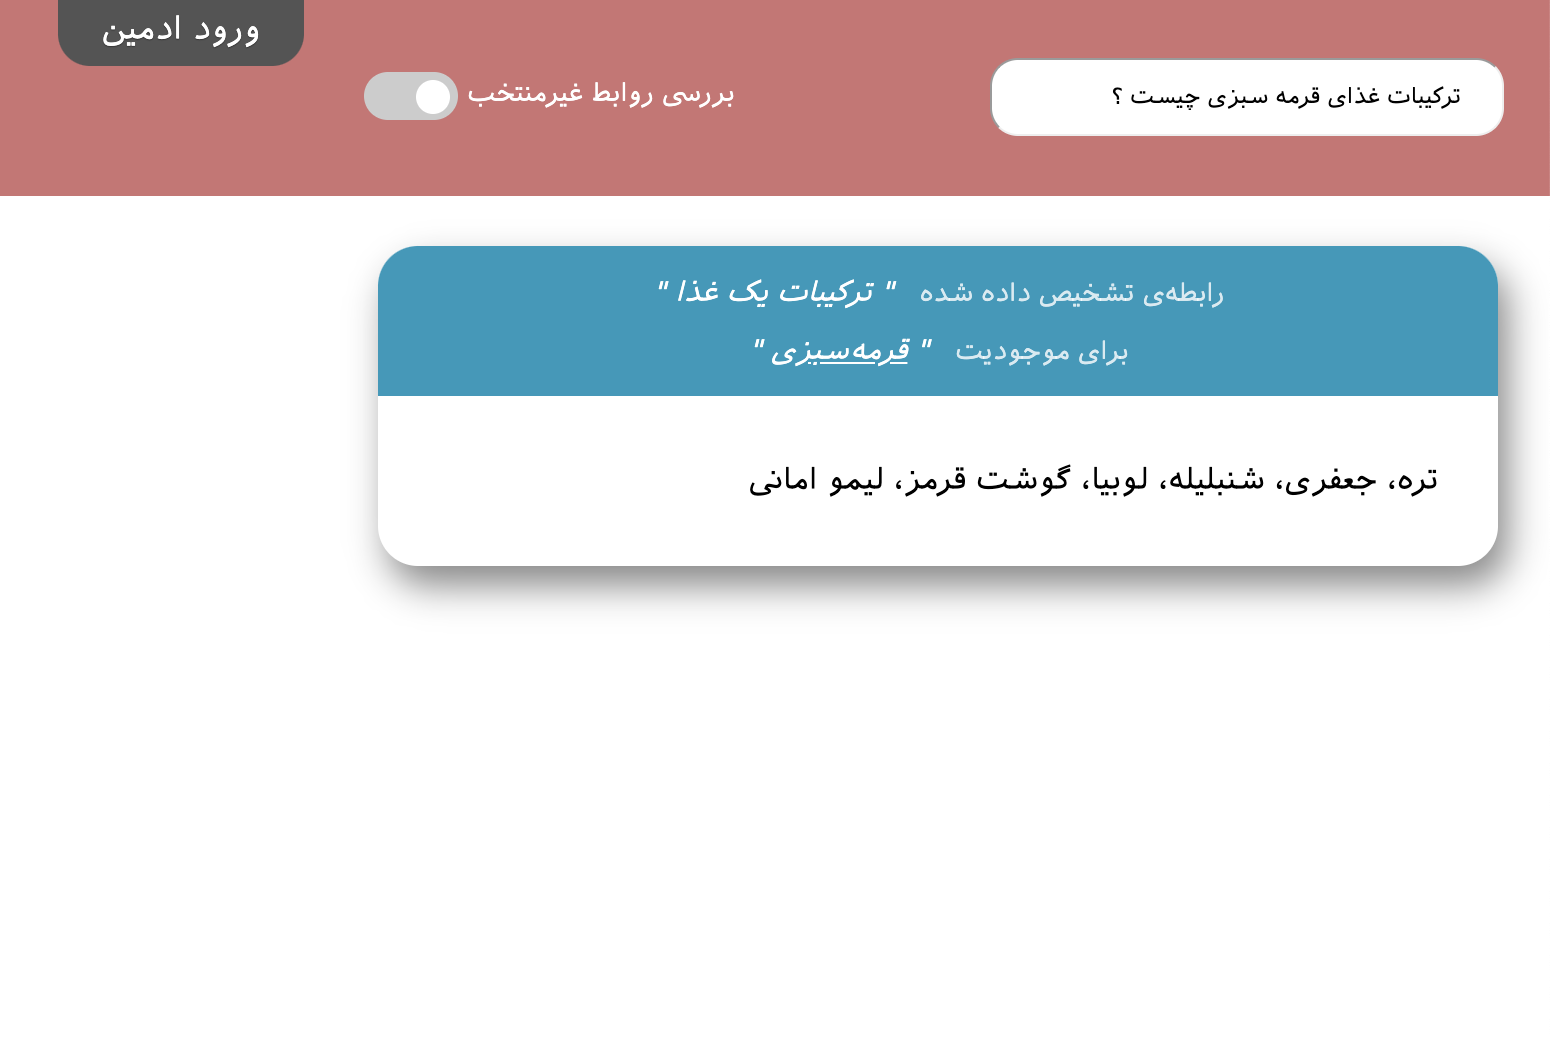
\includegraphics[width=15cm]{figures/interface/user.png}
	\caption{صفحه کاربر عادی}
\end{figure}
\vfill
\begin{figure}
	\centering
	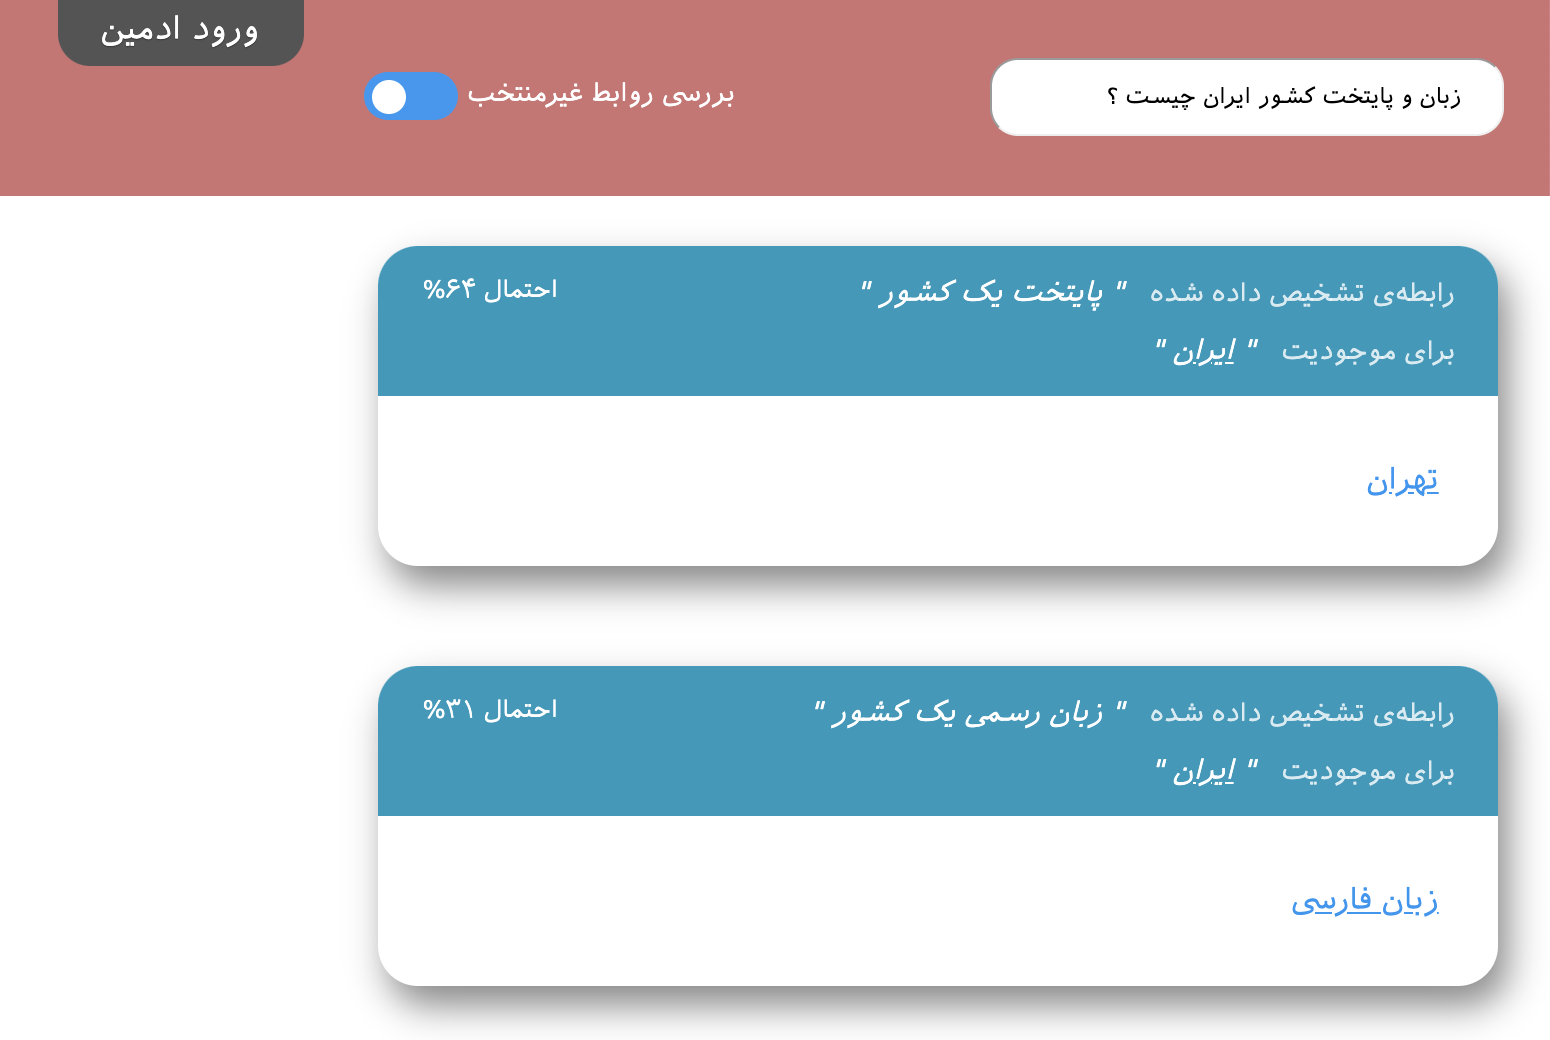
\includegraphics[width=15cm]{figures/interface/user-multiple-rel.png}
	\caption{صفحه کاربر عادی همراه روابط غیرمنتخب}
\end{figure}

\begin{figure}
	\centering
	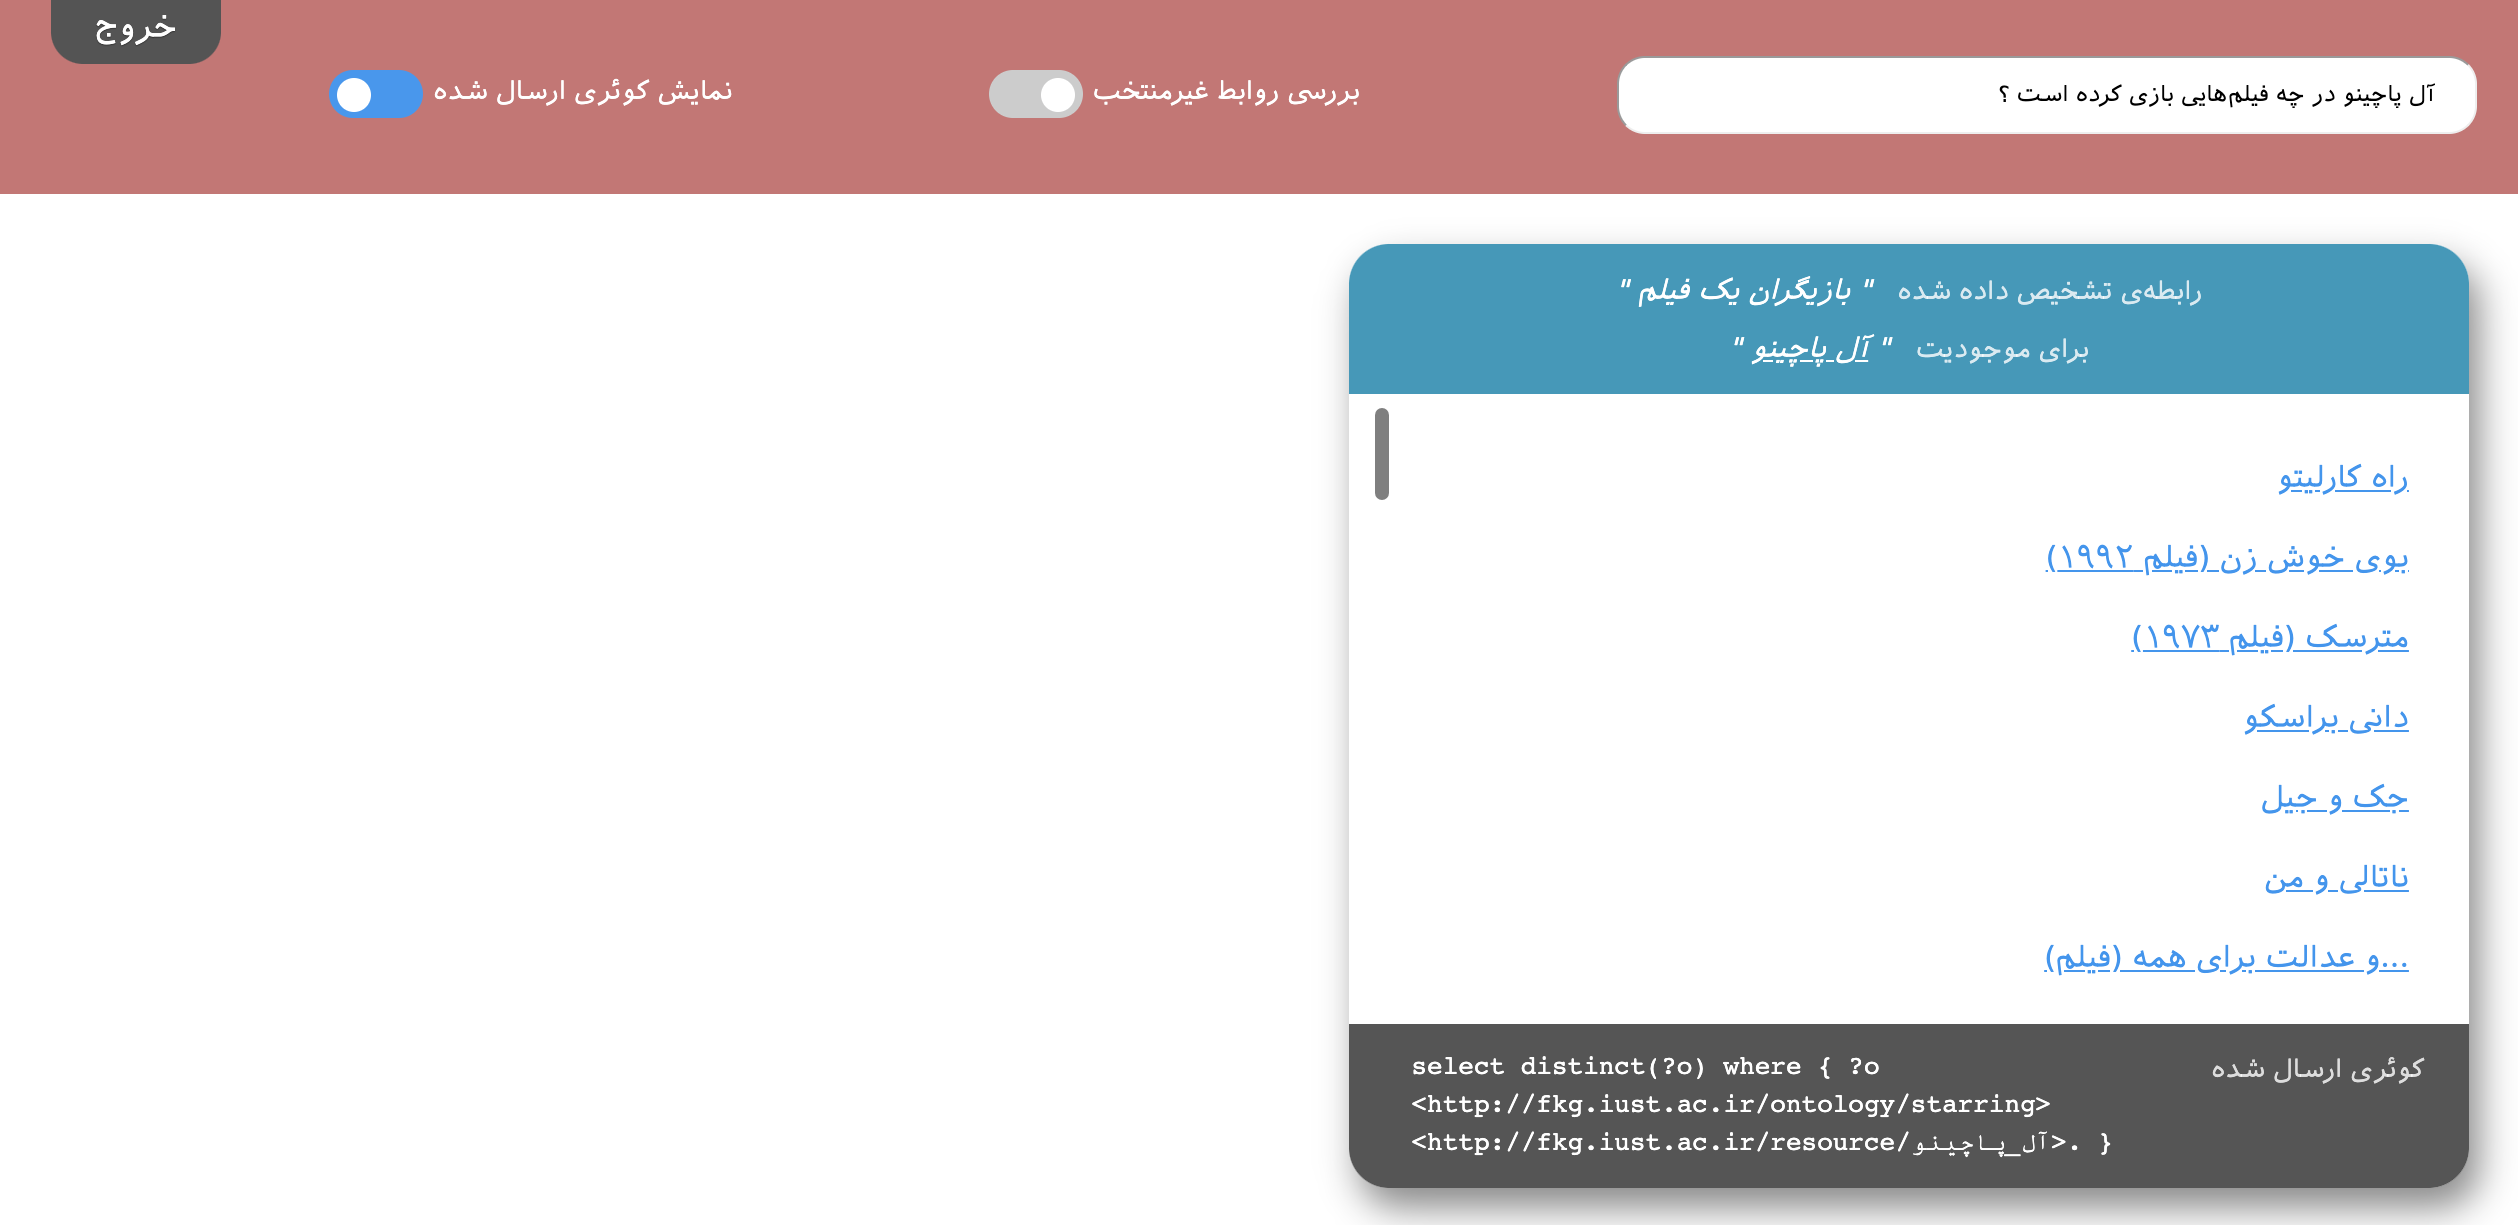
\includegraphics[width=15cm]{figures/interface/admin.png}
	\caption{صفحه کاربر تحلیل‌گر}
\end{figure}

\begin{figure}
	\centering
	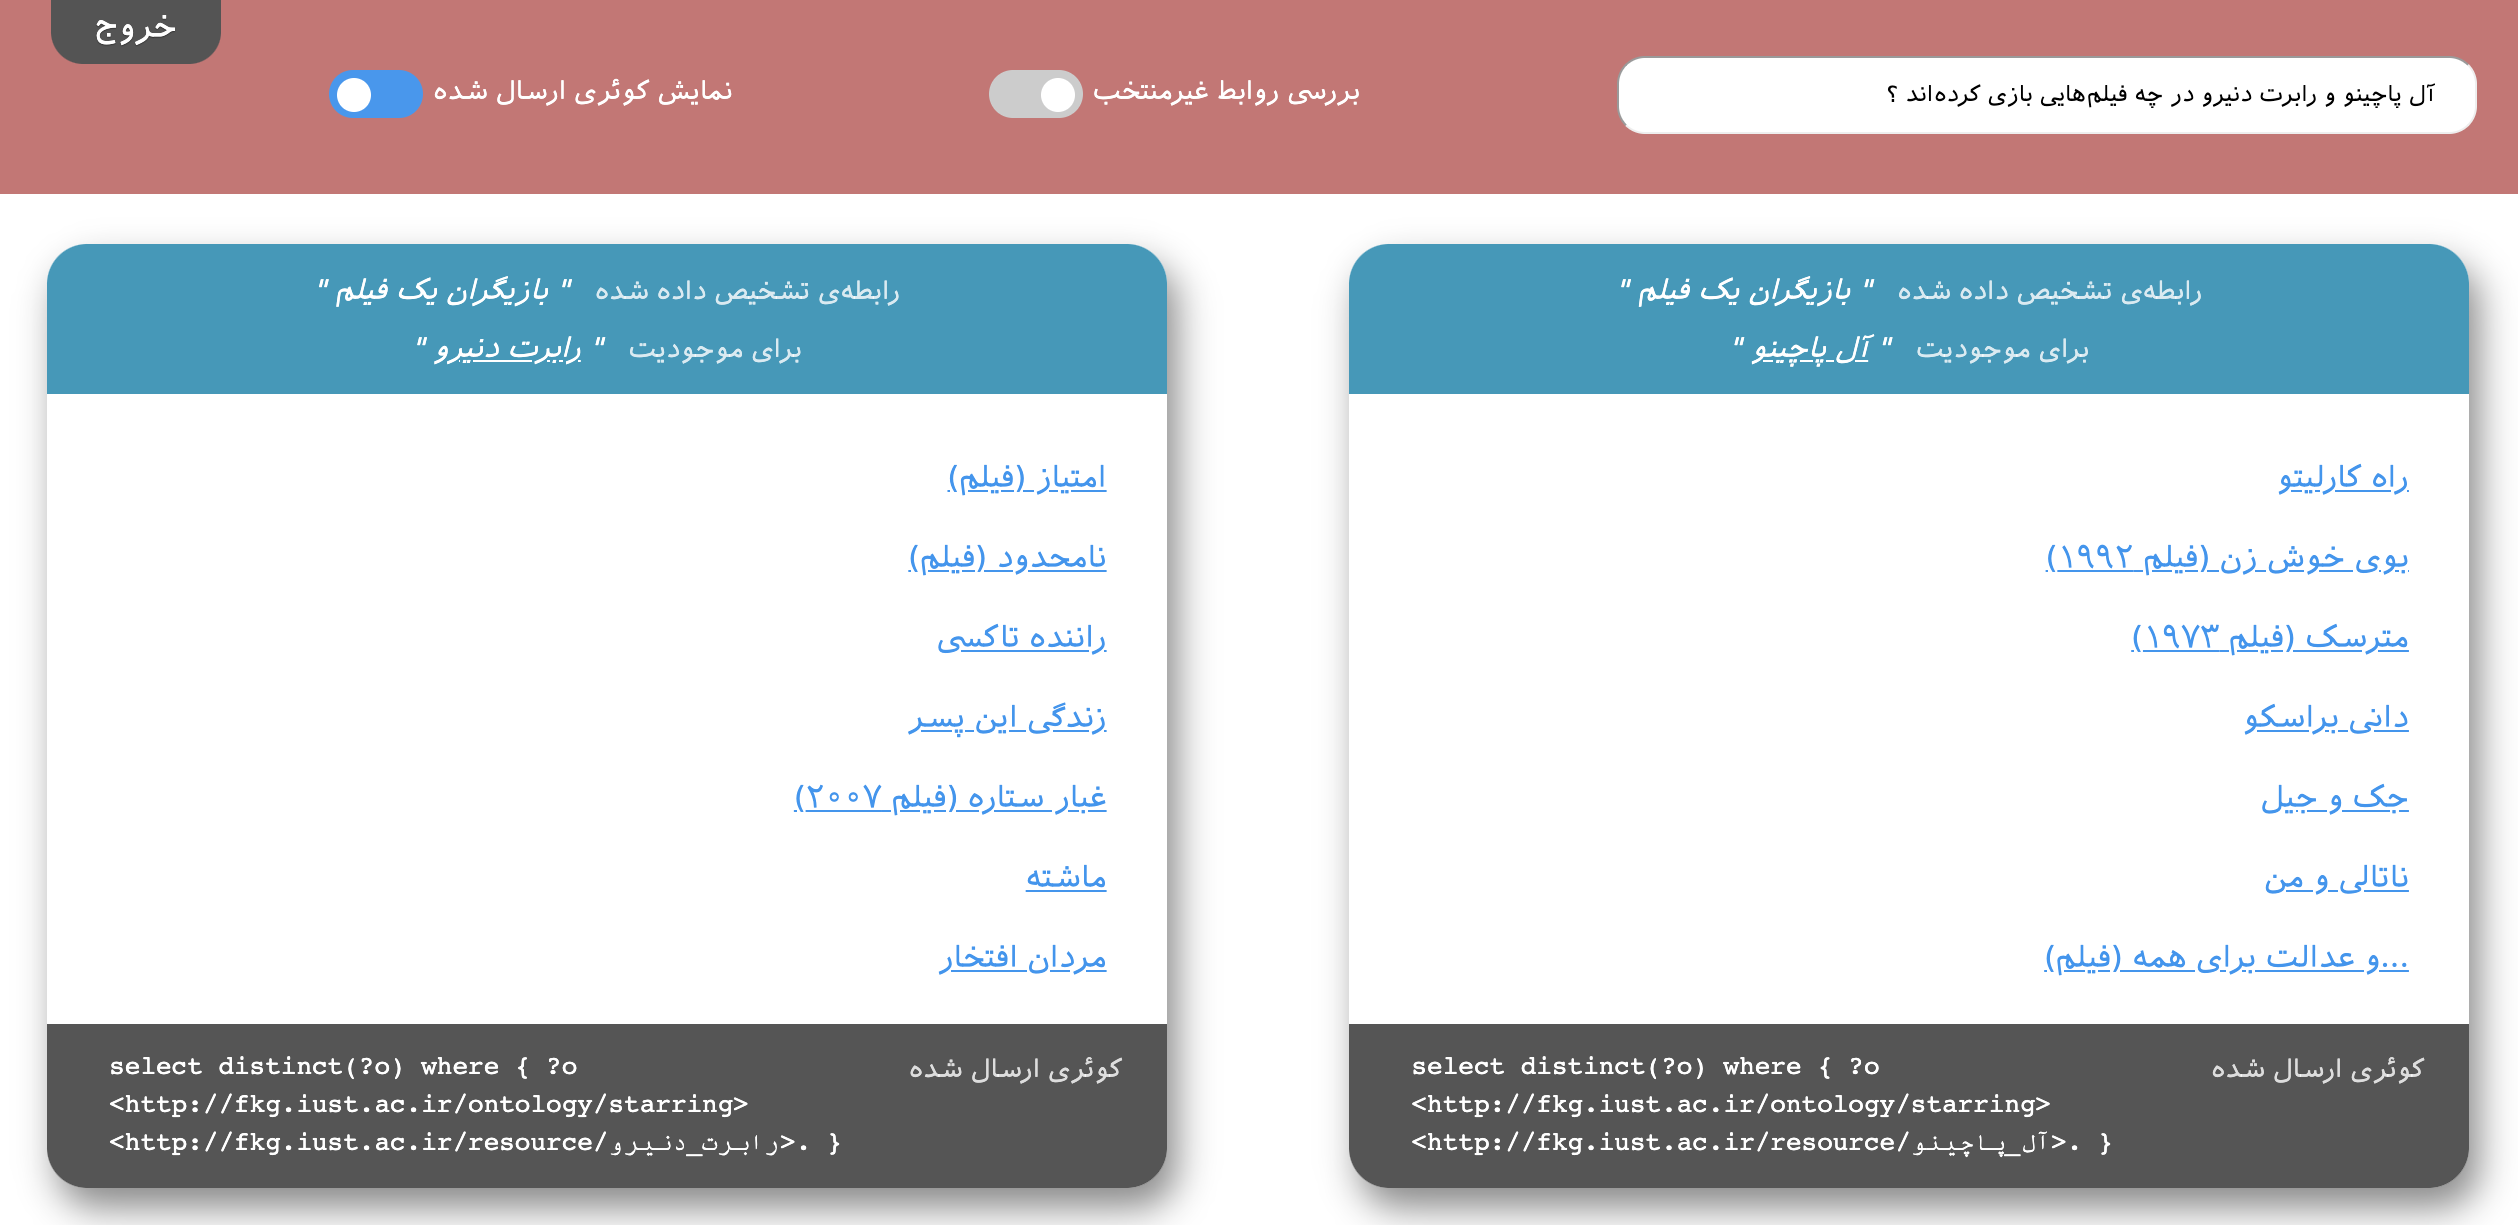
\includegraphics[width=15cm]{figures/interface/admin-multiple-ent.png}
	\caption{صفحه کاربر تحلیل‌گر همراه چند موجودیت}
\end{figure}

\begin{figure}
	\centering
	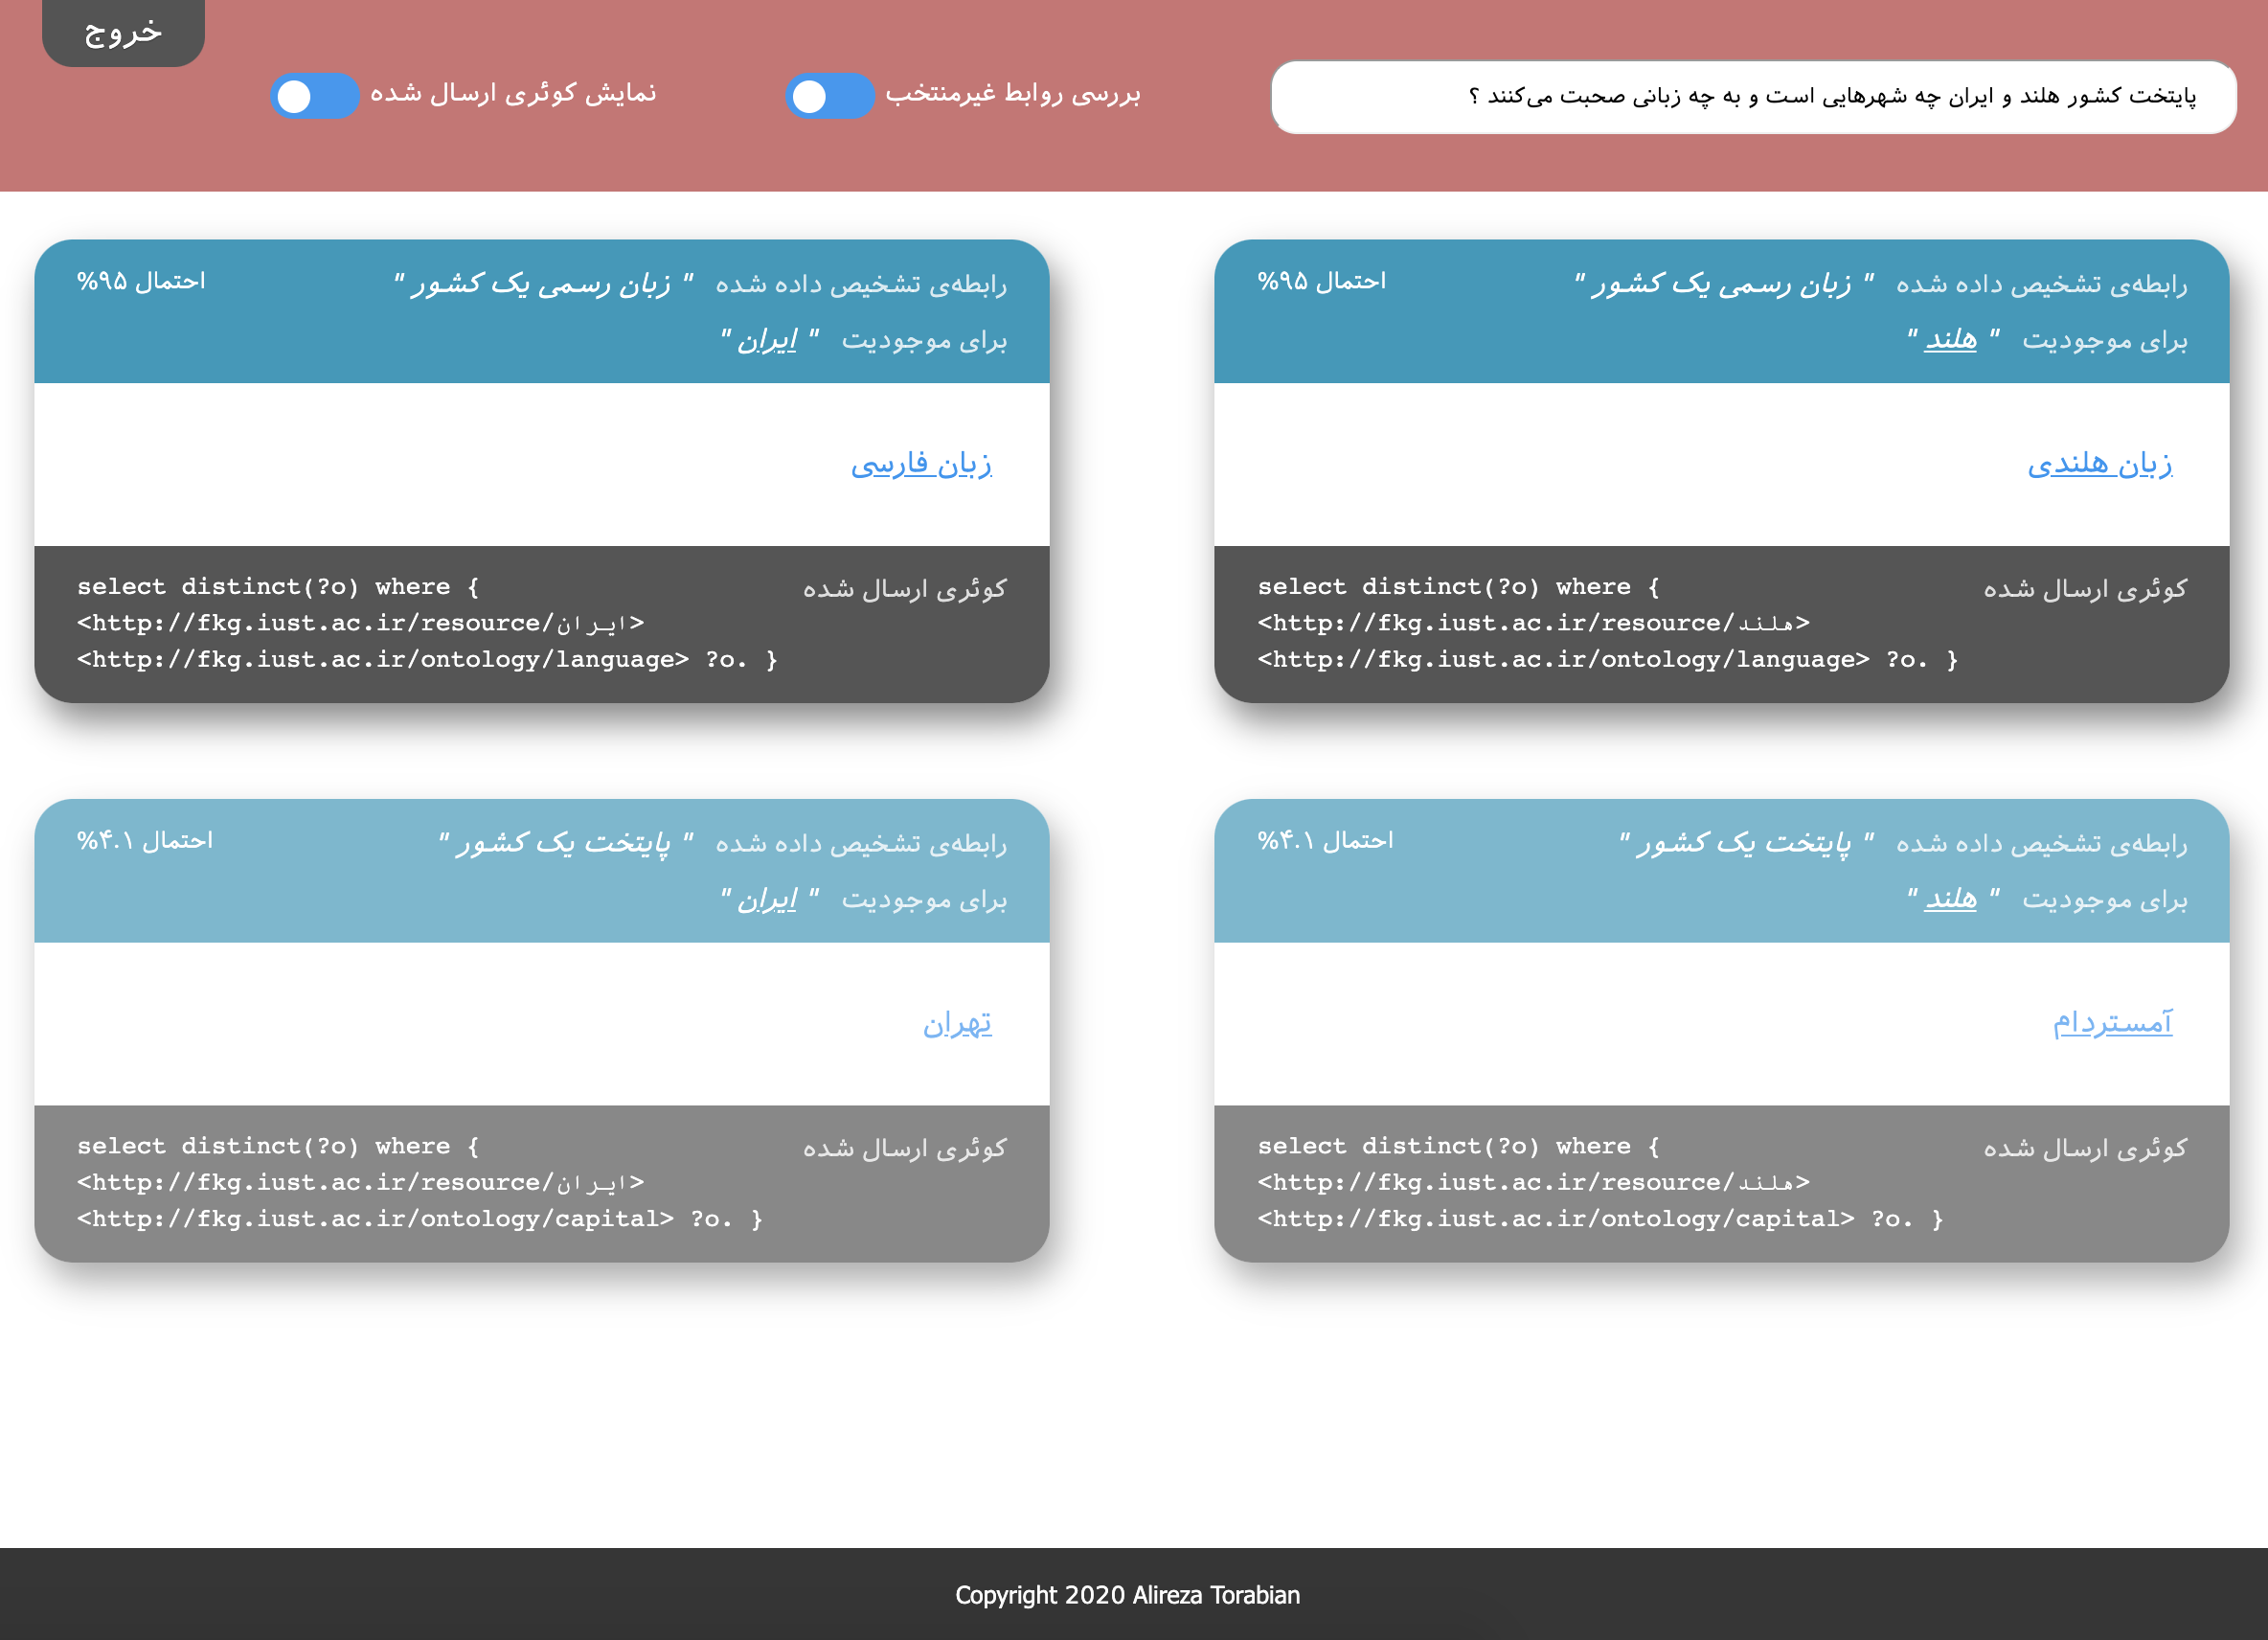
\includegraphics[width=15cm]{figures/interface/admin-double-multiple.png}
	\caption{صفحه کاربر تحلیل‌گر همراه چند موجودیت و روابط غیرمنتخب}
\end{figure}